\section{Our Proposal}

\subsection{Preliminaries}
These definitions, abstractions and techniques are used:
\begin{itemize}
\item \textbf{Semantic Network}: Consists of the tourism ontology extended with user's preferences and context factors. There is a semantic network for each user.
\item \textbf{Spreading Activation}: It is an algorithm able to take advantage of the hierarchical shape of the ontology (a Directed Acyclic Graph or DAG is formed) to propagate information related to the preferences over the different \textit{classes} of the semantic network.
\item \textbf{Aging}: To increment recommendation \textit{serendipity} \cite{kotkov2016survey}, each Point of Interest or POI will age for a user each time it is recommended to them.
\end{itemize}
The prototype system was built with Java. We used a Fuseki server as the triplestore, Apache Jena for traversing the ontology and connecting to the triplestore and a MySQL database for storing additional information of the nodes and items.

\begin{figure}[h]
\centering
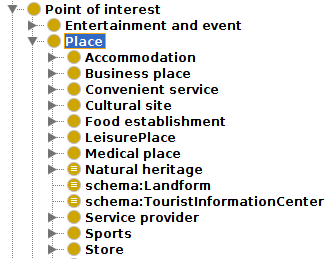
\includegraphics[scale=0.5]{ontology.png}
\caption{Subset of the modified version of the ontology DATATourisme (http://info.datatourisme.gouv.fr/ontology/core/2.0/)}
\label{fig:ontology}
\end{figure}

\subsection{Semantic Network} \label{section:semantic_network}

Based on \cite{bahramian_abbaspour_claramunt_2017}, the proposed system extends the nodes of an ontology with the following properties:
\begin{itemize}
    \item \textbf{Preference}: Real value in $[0, 1]$ that corresponds to the user rating for the node's ontology class.
    \item \textbf{Confidence}: Real value in $[0, 1]$ that defines how sure is the system about the user preference computed for the node. If the user explicitly specifies the preference of a node, the node's confidence should be $1$.
    \item \textbf{Activation}: Taking into account the user's context, this value determines how feasible it is to go to the kind of places that belong to the node's ontology class.
\end{itemize}{}
Both \textit{preference} and \textit{confidence} are \textbf{persistent} node attributes, while \textit{activation} is a \textbf{transient} node attribute. As told before, the extended ontology is called \textit{semantic network}, and there is one instance for each system user.

A subset of a modified version of the ontology DATATourisme (figure \ref{fig:ontology}) is used. The modification consists of specializing the original ontology class \textit{Sports and Leisure Place} into \textit{Sports} class and \textit{Leisure Place} class, hence making less ambiguous what kind of places should belong to that category. The subset consists of the \textit{Point of interest} class but only its \textit{Place} subclass, considering only the following \textit{Place}'s subclasses: \textit{Cultural Site, Food establishment, Leisure Place, Natural Heritage, Sports} and \textit{Store}. 

\subsubsection{Context factors} \label{section:context_factors}
As told before, \textit{context factors} are entities that describe the characteristics of the user's context that could affect their decision to go to a specific place. These factors are: 
\begin{itemize}
    \item \textit{Weather} (sunny/cloudless, rainy or snowy)
    \item \textit{Time} (early morning, morning, afternoon or night)
    \item \textit{Day} (weekday or weekend)
\end{itemize}
Following the ideas from \cite{bahramian_abbaspour_claramunt_2017}, these context factors are linked to a subset of "high level" ontology classes, that generalize enough our domain. These classes that are directly linked to the context factors are:
\begin{itemize}
    \item \textit{Museum}
    \item \textit{Interpretation Center}
    \item \textit{Library}
    \item \textit{Park and Garden}
    \item \textit{Archaeological Site}
    \item \textit{Religious Site}
    \item \textit{Remarkable Building}
    \item \textit{City Heritage}
    \item \textit{Defense Site}
    \item \textit{Remembrance Site}
    \item \textit{Technical Heritage}
    \item \textit{Food Establishment}
    \item \textit{Natural Heritage}
    \item \textit{Sports}
    \item \textit{Leisure Place}
    \item \textit{Store}
\end{itemize}
 
\subsection{Preferences propagation} \label{section:preferences-propagation}
Based on \cite{bahramian_abbaspour_claramunt_2017}, the steps for the preferences propagation are as follow:
\begin{enumerate}
    \item User gives a set of initial preferences for the classes that are mentioned on section \ref{section:context_factors}.
    
    \item Propagate preferences to the subclasses using formulas \ref{eq:preference} and \ref{eq:confidence}.
    
    \item Go back to step (1) if user wants to update preferences and start preferences propagation again from a specific node as source.
\end{enumerate}

\subsection{Context-awareness} \label{section:context-awareness}
Remembering the new definition of \textit{activation} on section \ref{section:semantic_network}, the formula \ref{eq:og_activation} is updated as follows:
\begin{equation} \label{eq:activation}
    act_c = \frac{\displaystyle \sum_{c' \in ancestors(c)} a_{c'}}{|ancestors(c)|}
\end{equation}
where $act_c$ is the activation for node $c$ and $ancestors(c)$ is the set of direct ancestors of node $c$. It could be seen as an averaged version of formula \ref{eq:og_activation} always using $w$ as $1$.

Let's define $f_x$ the \textit{fulfillment} of a context factor $x$ that has the value $1$ if $x$ fulfills or $0$ otherwise. Let's also define $r_{c,x}$ as the \textit{relevance} of context factor $x$ for node $c$, which is a real value in $[0, 2]$ that specifies how much the context factor can affect the decision to go to a POI that belongs to the node's ontology class; a value of $1$ means indifference; a value near $2$ means the fulfillment increases the wish to go to the POI; a value near $0$ means the fulfillment decreases the wish to go the POI. 

Now we define the activation for a node whose class $c$ is directly linked to the context factors (see section \ref{section:context_factors}):
\begin{equation} \label{eq:high_activation}
    act_c = \sum_{x \in contextFactors} r_{c,x} f_x
\end{equation}

Now we can define the steps for activation propagation as follow:
\begin{enumerate}
    \item The system receives information about the fulfillment of the context factors. For example, it receives the vector \textit{(sunny, early morning, weekend)}, stating that it is a sunny day, in the early morning on a weekend.
    
    \item Compute activation for classes that are directly linked to the context factors using formula \ref{eq:high_activation}.
    
    \item Propagate activation to subclasses using formula \ref{eq:activation}.
\end{enumerate}

\subsection{Recommender algorithm}

We will first give two necessary definitions to compute the final score of an item and then we give the formula for computing the final score.

\subsubsection{Aging}

Let's define $\eta_p$ as the POI $p$'s aging, initialized on $\eta_p = 1$. Let's define $H$ as the \textit{aging rate}. Each time a POI $p$ is recommended to the user, $\eta_p$ decreases by $H$. When $\eta_p < 0.1$, its aging value is reset to $1$. 

\subsubsection{Great-Circle distance}
Since the euclidean distance between two points on Earth would cross through the surface, we should use a more convenient measurement of distance: the \textit{great-circle distance} or \textit{orthodromic distance}. It is the shortest distance, along the surface of a sphere, between two points on the surface of the sphere. It is measured with circles on the sphere whose centers coincide with the center of the sphere. Those circles are called \textit{great-circles}. If we assume Earth is a perfect sphere and hence use Great-Circle distance, we get distances with errors no more than $0.5\%$ according to \cite{1997admiralty}. 

The distance between two points $i$ and $j$ on a sphere of radius $R$ is computed with the following formula:
\begin{equation} \label{eq:gc-dist}
    \begin{split}
        \scriptstyle{dist_{i,j} \ = \ R \cdot arccos (} & \scriptstyle{cos(lat_i) \cdot cos(lat_j) \cdot cos(lon_i - lon_j)} \\
                                        & \scriptstyle{+ \ sin(lat_i) \cdot sin(lat_j) )}
    \end{split}
\end{equation}

\subsubsection{Score} \label{section:score}
Let each $k_i$ be a parameter to the system, $dist_{u,p}$ be the great-circle distance between user $u$ and POI $p$ and $c$ be the node whose class is the one to which $p$ belongs. We define the \textit{score} of $p$ as a function that receives the maximum great-circle distance that a $p$ should be from $u$ as follows:
\begin{equation} \label{eq:score}
    \begin{split}
        score_p(maxdist) = \ &k_1 \cdot pref_c + k_2 \cdot act_c \\
                                        &+ k_3 \cdot \eta_p - k_4 \cdot \frac{dist_{u,p}}{maxdist}
    \end{split}
\end{equation}